%%%%%%%%%%%%%%%%%%%%%%%%%%%%%%%%%%%%%%%%%%%%%%%%%%%%%%%%%%%%%%%%%%%%%%%%%%%%%%
%
% タイトル TeX用テンプレート 
% バージョン 2014-11-8 (Sat) 初版
% 作成者 Kouhei Ito
% 作成場所 野々市市中林 DeuxMKK
% 用途 2段組レポートの作成等
%
%%%%%%%%%%%%%%%%%%%%%%%%%%%%%%%%%%%%%%%%%%%%%%%%%%%%%%%%%%%%%%%%%%%%%%%%%%%%%%%%
%\documentclass[11pt,twocolumn]{jsarticle}
\documentclass[11pt]{si2016}
\usepackage[dvipdfmx]{graphicx}
\usepackage{amsmath,amssymb}
\usepackage{url}
\usepackage{nidanfloat}

%% 体裁

% ページレイアウト(A4:297 mm × 210 mm,1 インチ = 25.4 mm)
% http://www.biwako.shiga-u.ac.jp/sensei/kumazawa/tex/layout.html
% http://www.slis.tsukuba.ac.jp/~fujisawa.makoto.fu/cgi-bin/wiki/index.php?TeX%A5%E1%A5%E2#p61e1b46
% 上 20 mm,下 22 mm,左右 20 mm の余白設定
\setlength{\topmargin}{-20truemm}
\setlength{\headheight}{10truemm}
\setlength{\headsep}{4.6truemm}
\setlength{\textheight}{255truemm}
\setlength{\oddsidemargin}{-5.4truemm}
\setlength{\evensidemargin}{-5.4truemm}  % twoside オプション指定時のみ有効
\setlength{\textwidth}{170truemm}
% \setlength{\columnsep}{8truemm}
\setlength{\columnsep}{6truemm}


%%%%%%%%%%%%%%%%%%%%%%%%%%%%%%%%%%%%%%%%%%%%%%%%%%%%%%%%%%%%%%%%%%%%%%%%%%%%%%%%
\title{カメラによるOpenCVを用いた3次元復元}
\author{金沢工業高等専門学校 佐々井翔也 戸澗健}
\date{2016-8-18}
%%%%%%%%%%%%%%%%%%%%%%%%%%%%%%%%%%%%%%%%%%%%%%%%%%%%%%%%%%%%%%%%%%%%%%%%%%%%%%%%
\begin{document}
\maketitle
\begin{abstract}
近年,自動車などを中心に自動運転技術が発展してきている.それに伴い画像処理によって自身の位置を認識する技術の需要が高まっている.そこで,今回は
OpenCV(正式名称: Open Source Computer Vision Library)という画像や動画を処理することに適しているオープンソースのコンピューター・ビジョン・ライブラリを用いて自身の位置を特定する仕組みを作成することを目的とする.
\end{abstract}

\tableofcontents
%%%%%%%%%%%%%%%%%%%%%%%%%%%%%%%%%%%%%%%%%%%%%%%%%%%%%%%%%%%%%%%%%%%%%%%%%%%%%%%%
\section{はじめに}
今回,つくばチャレンジに参加するためにロボットが自律走行を行う必要がある.そのため,自身の位置を認識する手段としてカメラを用いることにした.まず,カメラである利点として,安価である点,GPSが必要ない点,周りの状況がわかる点などが挙げられる.特に、周りの状況がわかることで障害物を回避し,その場でマッピングするなど幅広く活用できる.

%\section{開発環境}


\section{3次元復元}
3次元復元とは,画像上の2次元座標から3次元座標を得ることである.これは、カメラの焦点距離と画像のセンター座標を含む内部パラメータ行列を使用して行う.また,Mをカメラの内部パラメータ行列,[R|t]を並進・回転の同次変換行列としその関係式を下記に示す.
\begin{equation}
\left(
    \begin{array}{c}
      u \\
      v \\
      1 
    \end{array}
  \right)=M[R|t]\left(
    \begin{array}{c}
      X \\
      Y \\
      Z \\
      W
    \end{array}
  \right)
\end{equation}
実際の3次元座標はXYZをそれぞれWで割ることにより求まる.

3次元復元の流れを下記に示す.

\subsection{カメラの校正}
\subsubsection{カメラの校正}
カメラの校正とはレンズによって生じる歪みやレンズの焦点距離などのパラメータを推定するものであり,OpenCVの校正アルゴリズムではピンホールカメラモデルを想定している.

\subsubsection{ピンホールカメラモデル}
ピンホールカメラとはピンホール(光学中心)を開けた箱の内側に外界の風景を上下左右反転して映ることを利用した初期のカメラである.そして,ピンホールを通る光線だけで投影面への結像をモデル化したのがピンホールカメラモデルであり,そのモデルを図1に示す.

\begin{figure}[b]
 \begin{center}
  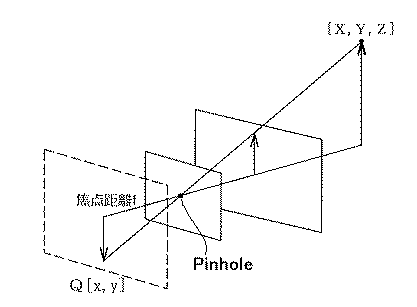
\includegraphics[width=80mm]{pinhole.png}
  \caption{ピンホールカメラモデル}%図題
  \label{fig:02}%文章中の名前
 \end{center}
\end{figure}

図1よりピンホールを通過した光線は画像面の1点と交わり,そこで像を結ぶ.この像は元の画像を逆転させたものになるため画像面を光学中心より前に移すと良い.また画像面を移すことを透視投影と呼ぶ.

\subsubsection{透視変換}
カメラの結像に関する座標系を図2,カメラと画像の座標系を図3に示す.

\begin{figure}[b]
 \begin{center}
  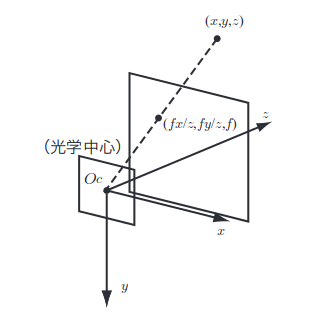
\includegraphics[width=80mm]{camera1.png}
  \caption{カメラの結像に関する座標系}%図題
  \label{fig:02}%文章中の名前
 \end{center}
\end{figure}

\begin{figure}[b]
 \begin{center}
  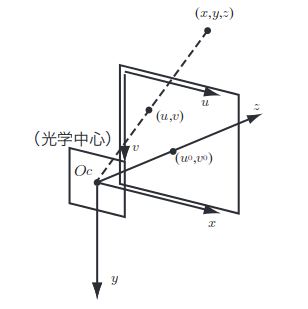
\includegraphics[width=80mm]{camera2.png}
  \caption{カメラと画像の座標系}%図題
  \label{fig:02}%文章中の名前
 \end{center}
\end{figure}

光学中心Ocから画像面までの距離(焦点距離)をfとすると,
この座標系で(x,y,z)にある空間の点に対応する像は相似の関係(fx/z,fy/z,f)となる.
画像面上の点(fx/z,fy/z)の透視変換は

\begin{equation}
\left(
    \begin{array}{c}
      x \\
      y \\
      z 
    \end{array}
  \right)=\frac{f}{z} \left(
    \begin{array}{c}
      x \\
      y \\
       
    \end{array}
  \right)
\end{equation}
となる.つまり,カメラに対する相対的な位置によって,結像される位置が決まる.

\subsection{Essential Matrixを求める}
Essential Matrixとは2つのカメラを実空間で関連付ける,平行移動と回転に関する情報を含む行列である.また,Essential Matrixを下記に示す.

\begin{equation}
       Essential Matrix = \left(
    \begin{array}{cccc}
      r _{11} & r _{12} & r _{13} & t_1\\
      r _{21} & r _{22} & r _{23} & t_2\\
      r _{31} & r _{32} & r _{33} & t_3\\

    \end{array}
  \right)
\end{equation}
OpenCVでEssential Matrixを求める際に利用されている手法は8点法{\scriptsize[1]}もしくはその改良版の5点法である.
カメラのパラメータが既知の場合,5点法を用いることでEssential Matrixを求めることができる.


\subsection{回転行列・並進行列を求める}
回転行列Rは3×3,並進行列tは3×1の行列で表される.
式3よりEssential Matrixは回転行列Rと並進行列tを1つにまとめた4×4の行列[R|t]で構成されていることが分かる.よってEssential Matrixを分解することにより,回転行列Rと並進行列tを求めることができる.

\subsection{三角測量}
対応付けされた2点間の座標と並進,回転を求めることで図4のように二次元座標を三次元復元することができる.

\begin{figure}[b]
 \begin{center}
  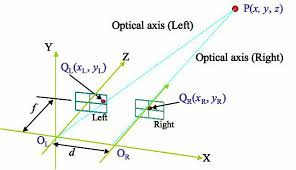
\includegraphics[width=80mm]{index.jpeg}
  \caption{三角測量}%図題
  \label{fig:01}%文章中の名前
 \end{center}
\end{figure}

左画像の中心Q{\scriptsize L},右画像の中心Q{\scriptsize R},特徴点Pをつなげることで三角形を作ると,特徴点Pの座標は式4,式5,式6のような関係が成り立つ.

\begin{equation}
 x=\frac {d・x_{L}}{X_{L}-X_{R}}
\end{equation}

\begin{equation}
 y=\frac {d・y_{L}}{X_{L}-X_{R}}
\end{equation}

\begin{equation}
 z=\frac {d・f}{X_{L}-X_{R}}
\end{equation}


式4,式5,式6より,特徴点Pの三次元座標を得ることができる.


\section{つくばチャレンジについて}
つくばチャレンジでは,自律走行を行うことを目標にしている.また,自律走行を行うためにはロボットが自分の位置を認識する必要がある.そこで,3次元復元で得られた座標情報から周囲の地図を作成すると同時に現在の位置を過去の地図データと照らし合わせて認識することにした.


\section{終わりに}
3次元復元を行い得られた座標情報は,対応付けられた点情報とカメラの内部パラメータが正確であれば正しいといえる.さらに,座標情報が正確であれば地図データや現在の位置も正確に求まる.また,カメラの内部パラメータは校正により求まる.よって,対応付けられた点情報の正確性を高めることが最も重要であると言える.
\section{参考文献}
[1]Bradski,Kaehler:詳解 OpenCV,433,株式会社オライリー・ジャパン(2012)


%%%%%%%%%%%%%%%%%%%%%%%%%%%%%%%%%%%%%%%%%%%%%%%%%%%%%%%%%%%%%%%%%%%%%%%%%%%%%%%%


\end{document}
